

\clearpage
\subsection{The Pottery merchant}
\label{sec:appendix:moj:pottery}

A Viking potter was called a leirkerasmithr. Archaeologists can now work out what individual pots were specifically used for, providing insights into Viking diet, trade and migration.

\begin{display}{The pottery stall}
	\label{fig:appendix:moj:places:pottery:stall}
	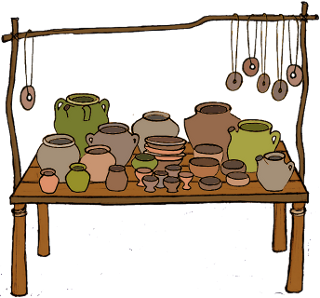
\includegraphics[width=0.65\columnwidth]{img/Jorvik/places/pottery stall}
\end{display}

\begin{display}{The pottery stall with a background and a merchant}
	\label{fig:appendix:moj:places:pottery}
	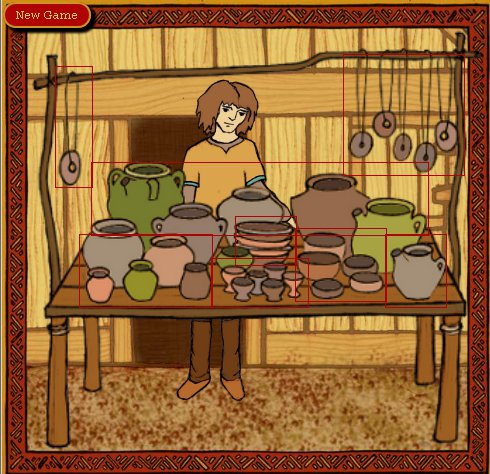
\includegraphics[width=0.65\columnwidth]{img/Jorvik/places/pottery}
\end{display}
\clearpage


\begin{table}[ht!]
	\centering
	\begin{tabular}{ p{3cm} c }\toprule
		\textbf{Name:} & \multirow{5}{*}{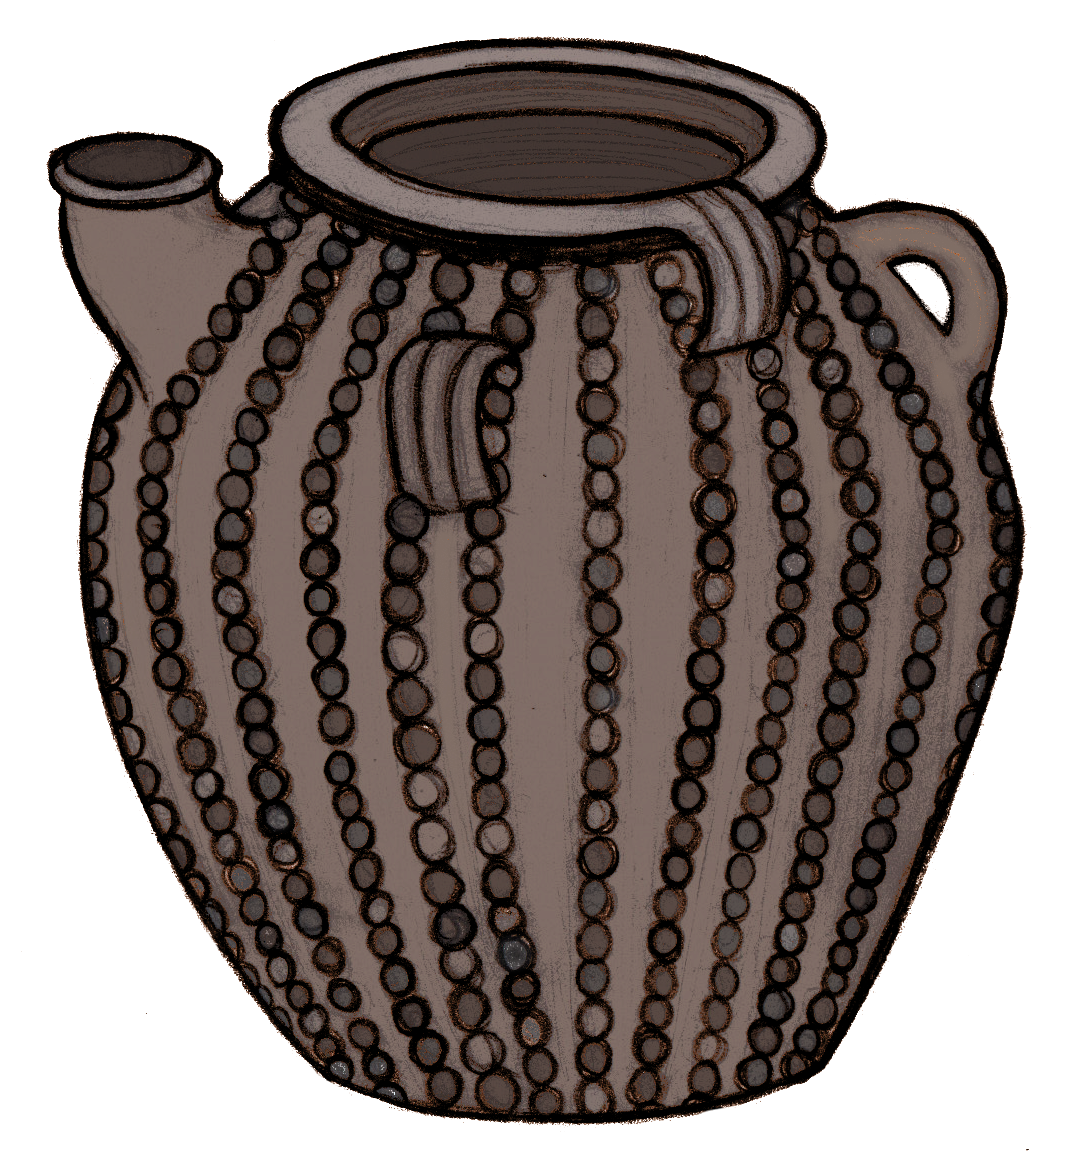
\includegraphics[height=30mm]{img/Jorvik/objects/pottery/jug}}\\
		Jug & \\ 
		\textbf{Price:} & \\
		2.20 Silver. & \\ 
		\textbf{Description:} & \\
		\multicolumn{2}{p{12cm}}{Clay jugs were used to serve drinks. Vikings also used bottles made out of wood, clay or leather.}\\
		\bottomrule
	\end{tabular}
\end{table}

\begin{table}[ht!]
	\centering
	\begin{tabular}{ p{3cm} c }\toprule
		\textbf{Name:} & \multirow{5}{*}{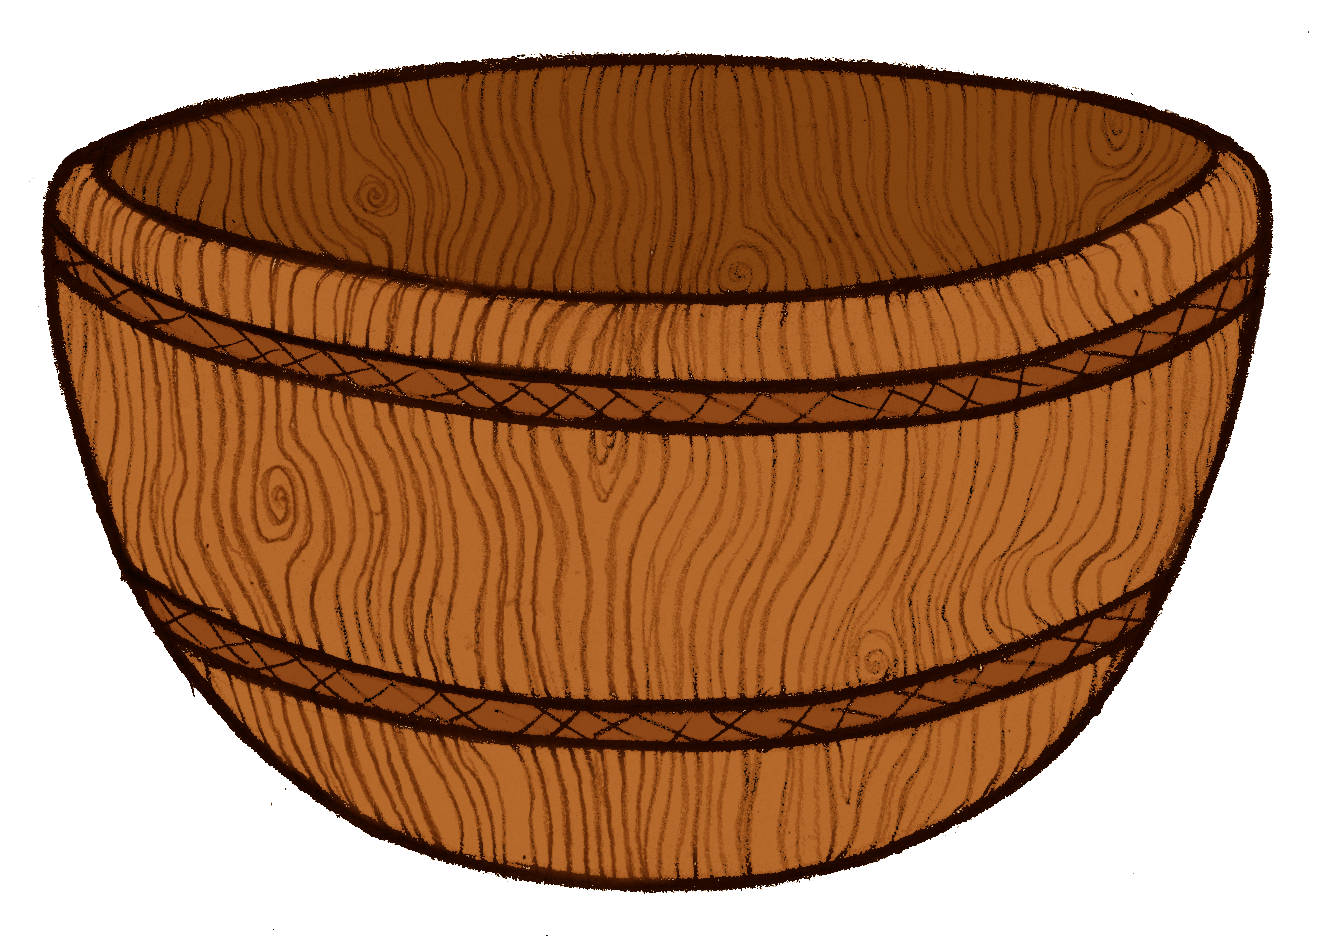
\includegraphics[height=30mm]{img/Jorvik/objects/pottery/bowl}}\\
		Bowl & \\ 
		\textbf{Price:} & \\
		0.88 Silver. & \\ 
		\textbf{Description:} & \\
		\multicolumn{2}{p{12cm}}{Bowls were made from wood and sometimes clay. Well-preserved Viking bowls could easily be mistaken for being modern.}\\
		\bottomrule
	\end{tabular}
\end{table}

\begin{table}[ht!]
	\centering
	\begin{tabular}{ p{3cm} c }\toprule
		\textbf{Name:} & \multirow{5}{*}{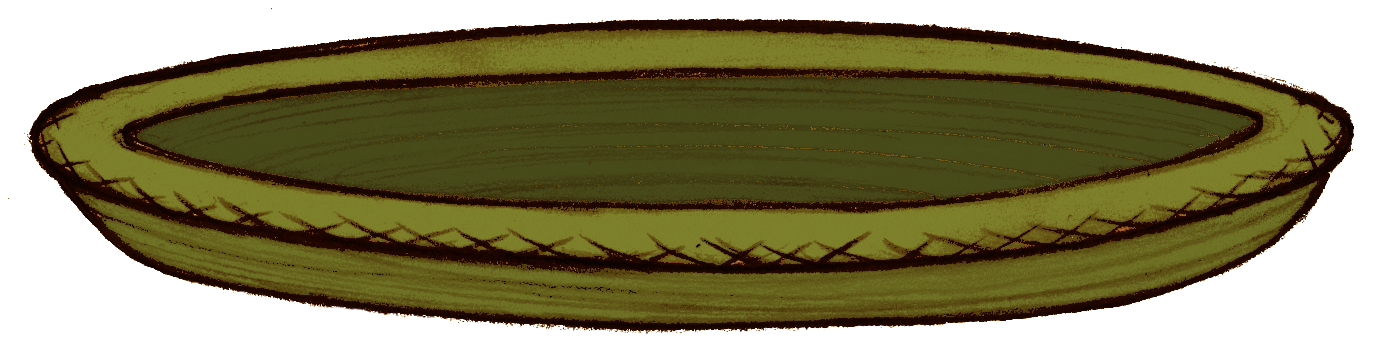
\includegraphics[width=70mm]{img/Jorvik/objects/pottery/plate}}\\
		Plate & \\ 
		\textbf{Price:} & \\
		0.88 Silver. & \\ 
		\textbf{Description:} & \\
		\multicolumn{2}{p{12cm}}{Vikings plates would have been made out of wood and occasionally out of clay. They would be made in a variety of different sizes.}\\
		\bottomrule
	\end{tabular}
\end{table}

\begin{table}[ht!]
	\centering
	\begin{tabular}{ p{3cm} c }\toprule
		\textbf{Name:} & \multirow{5}{*}{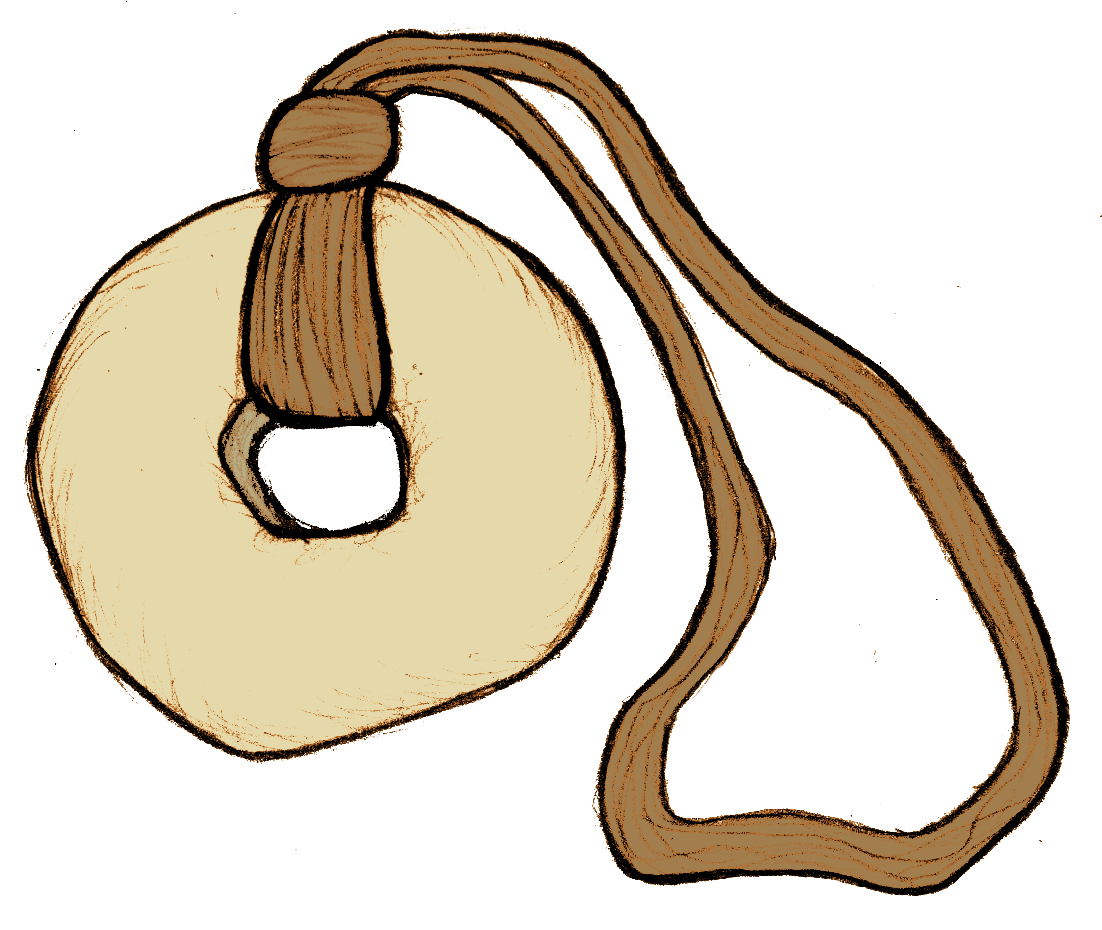
\includegraphics[height=30mm]{img/Jorvik/objects/pottery/loom weights}}\\
		Loom Weights & \\ 
		\textbf{Price:} & \\
		0.44 Silver. & \\ 
		\textbf{Description:} & \\
		\multicolumn{2}{p{12cm}}{Clay weights were important in the construction of a warp-weighted loom. This invention was one of two ways that both Viking men and women could weave cloth.}\\
		\bottomrule
	\end{tabular}
\end{table}

\begin{table}[ht!]
	\centering
	\begin{tabular}{ p{3cm} c }\toprule
		\textbf{Name:} & \multirow{5}{*}{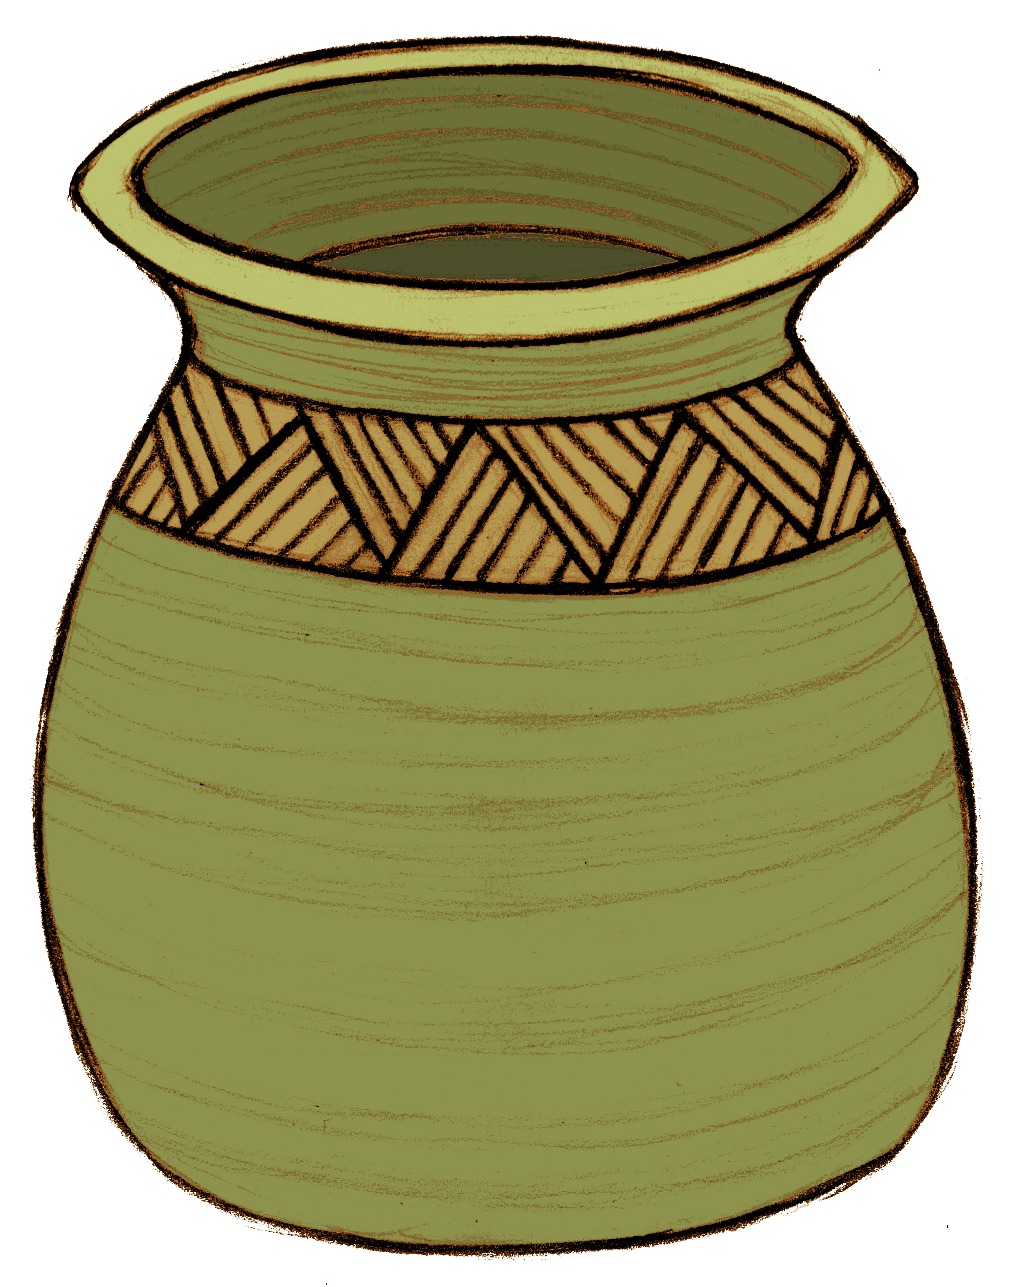
\includegraphics[height=30mm]{img/Jorvik/objects/pottery/cooking pots}}\\
		Cooking Pots & \\ 
		\textbf{Price:} & \\
		1.32 Silver. & \\ 
		\textbf{Description:} & \\
		\multicolumn{2}{p{12cm}}{Viking pots had a number of uses including cooking, storage and serving meals. Pottery tended to be grey, sometimes shell-tempered when broken oyster shells were mixed into the clay.}\\
		\bottomrule
	\end{tabular}
\end{table}

\begin{table}[ht!]
	\centering
	\begin{tabular}{ p{3cm} c }\toprule
		\textbf{Name:} & \multirow{5}{*}{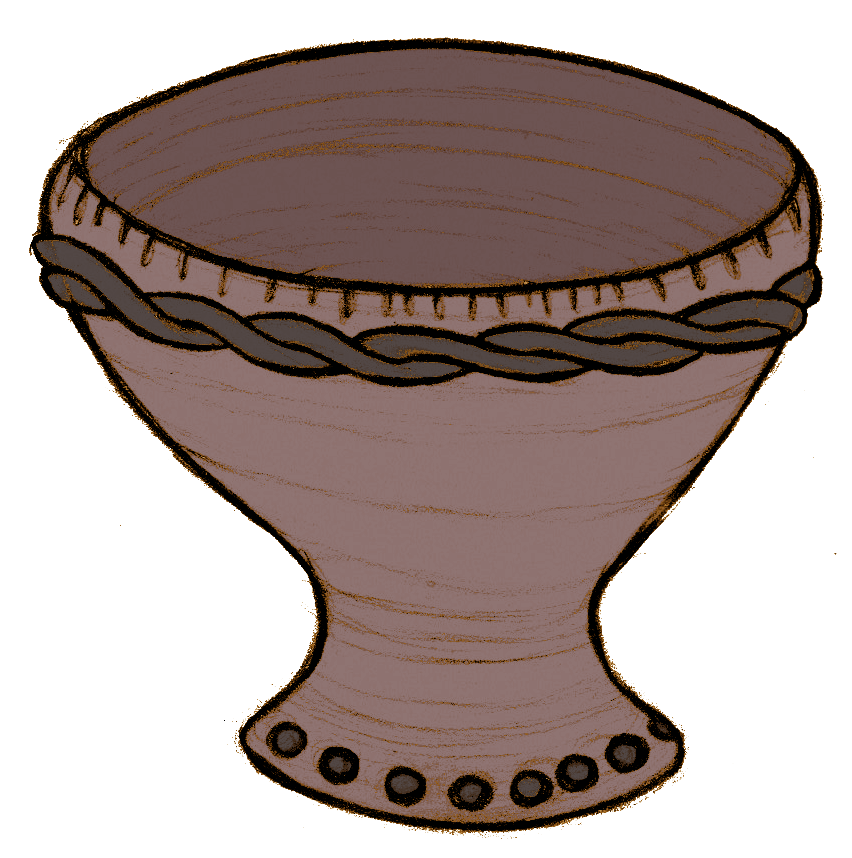
\includegraphics[height=30mm]{img/Jorvik/objects/pottery/oil lamps}}\\
		Oil Lamps & \\ 
		\textbf{Price:} & \\
		0.88 Silver. & \\ 
		\textbf{Description:} & \\
		\multicolumn{2}{p{12cm}}{Oil lamps provided the only light source in Viking homes besides the central hearth and the natural light through small windows during the day. The lamps were made of clay or carved from soapstone.}\\
		\bottomrule
	\end{tabular}
\end{table}